%%%%%%%%%%%%%%%%%%%%%%%%%%%%%%%%%%%%%%%%%%%%%%%%%%%%%%%%%%%%%%%%%%%%%%%%%%%%
%  第16回 例題8〜10（原本 20161215143926.pdf の p75/p76/p77 より）
%  原本は「問題枠 →(指針)空欄→【KEY】」で解答が載っていないため，
%  【指針】と【解答】は本文の説明・練習問題の解答の解き方に合わせて書き起こした．
%  （例題10 の指針だけは原本にも(5)についての記述があるので，それを含めてある）
%  ※ このファイルは記録用。実体は physics_ch16.tex に流し込み済み。
%%%%%%%%%%%%%%%%%%%%%%%%%%%%%%%%%%%%%%%%%%%%%%%%%%%%%%%%%%%%%%%%%%%%%%%%%%%%

%%%%%%%%%%%%%%%%%%%%  例題8（16.2 の直後）  %%%%%%%%%%%%%%%%%%%%
\begin{reidaiunit}
\begin{reidai}{気体のした仕事}
\begin{zuright}{68mm}
\hspace{1zw}図のように断面積$S\U{m^2}$のシリンダーに気体を封入し，ピストンに図のように弾性定数が$k\U{N/m}$のバネを取り付けた．バネが自然長のとき，ちょうど大気圧$P_0\U{Pa}$とシリンダー内の気体の圧力とがつり合った．シリンダー内のヒーターから少しずつ気体を加熱していったところ，気体はゆっくりと膨張し，ピストンはゆっくりと距離$a\U{m}$だけ進んだという．図のように$x$軸を取り，その原点をピストンの初期位置として以下の問に答えよ．
\zusep
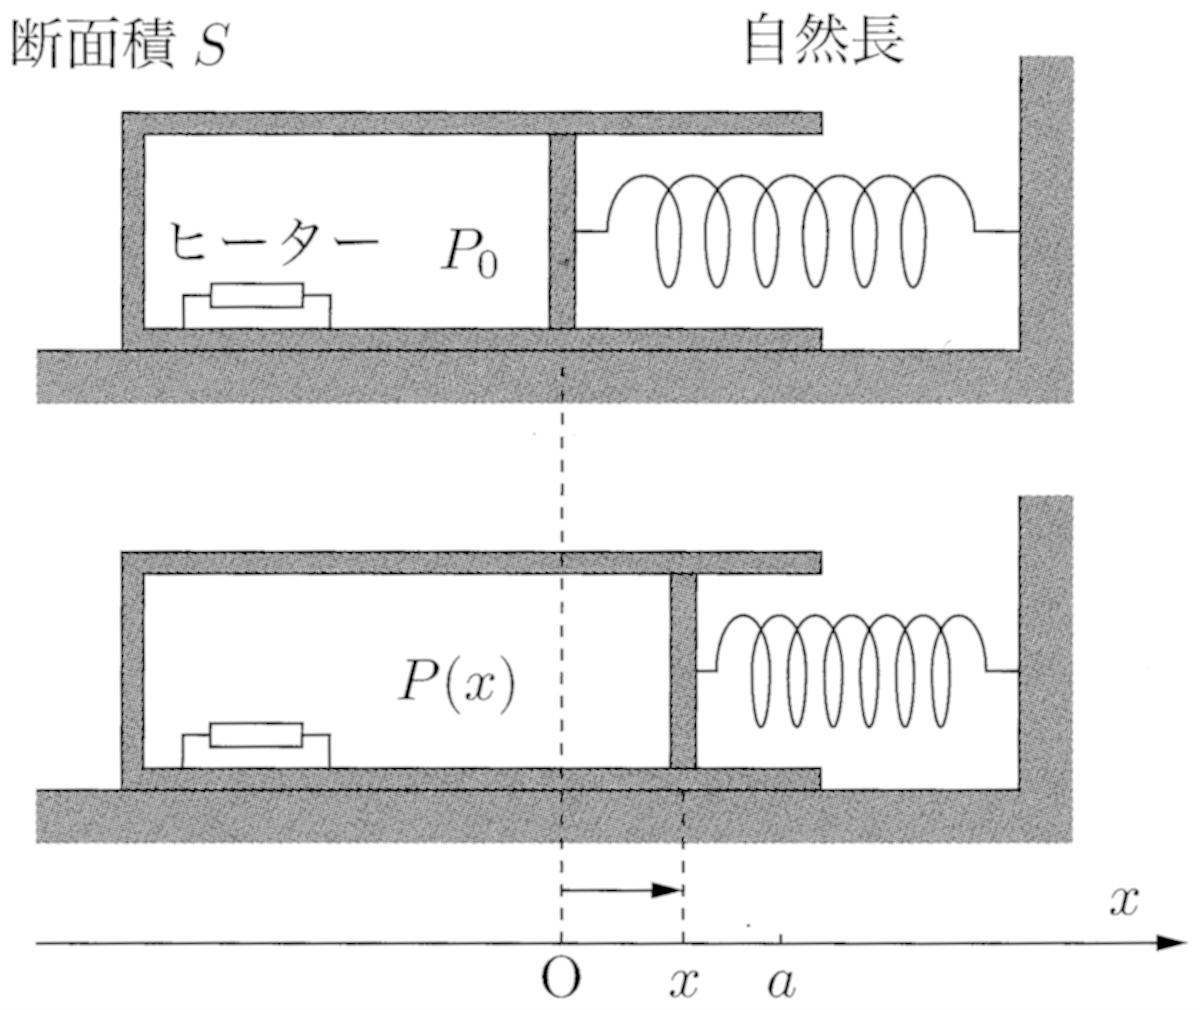
\includegraphics[keepaspectratio,width=68mm]{fig/ch16_ex8_cyl.png}
\end{zuright}
\begin{komon}
\ko{1} ピストンが位置$x\U{m}$にあるときの気体の圧力$P(x)\U{Pa}$を求めよ．
\ko{2} ピストンが$x\U{m}$から微小距離$x+dx\U{m}$だけ移動する間に気体が外界に対してする仕事$dw\U{J}$を求めよ．
% 原本の文言のまま．正確には「位置 x[m] から x+dx[m] まで移動する間に」の意．
\ko{3} この変化の$P-V$図を描け．ただし，$x=0\U{m}$のときの気体の体積を$V_0\U{m^3}$とする．
\ko{4} この状態変化で気体が外界に対してする全仕事$w\U{J}$を求めよ．
\end{komon}
\end{reidai}

\begin{sisinE}
ゆっくりと変化させているので，各瞬間でピストンに働く力はつり合っている．ピストンに働くのは，気体の圧力による力，大気圧による力，バネの弾性力の三つである．気体の圧力$P(x)$はこのつり合いの式から求まる．

体積と$x$は$V=V_0+Sx$，したがって$dV=S\,dx$で結ばれるので，$w=\displaystyle\int P\,dV$は$x$についての積分に書き換えて計算するとよい．
\end{sisinE}

\Key{ゆっくり変化させる $\Rightarrow$ ピストンはつり合いを保ちつつ変化する\quad $dw=P\,dV \rightarrow w=\displaystyle\int_{V_1}^{V_2}P\,dV$}

\begin{kaitou}
\begin{komon}
\ko{1} ピストンが位置$x$にあるとき，バネは自然長から$x$だけ縮んでおり，ピストンを左向きに$kx\U{N}$の力で押す．ピストンに働く力のつり合いより，
       \Ana{P(x)S=P_0S+kx}
       よって，
       \Ana{P(x)=P_0+\frac{kx}{S}\U{Pa}\Ans}
\ko{2} ピストンが$dx$だけ移動する間の気体の体積増加は$dV=S\,dx$であるから，
       \Ana{dw=P(x)\,dV=\left(P_0+\frac{kx}{S}\right)S\,dx=(P_0S+kx)\,dx\U{J}\Ans}
\ko{3} 気体の体積は$V=V_0+Sx$，すなわち$x=\dfrac{V-V_0}{S}$であるから，これを(1)に代入して
       \Ana{P=P_0+\frac{k(V-V_0)}{S^2}}
       となり，$P$は$V$の一次関数である．$x:0\rightarrow a$の変化であるから，体積は$V_0\rightarrow V_0+aS$，圧力は$P_0\rightarrow P_0+\dfrac{ka}{S^2}$と変化する．よって$P-V$図は次図．
       \begin{center}
       \ifbsAnaume
       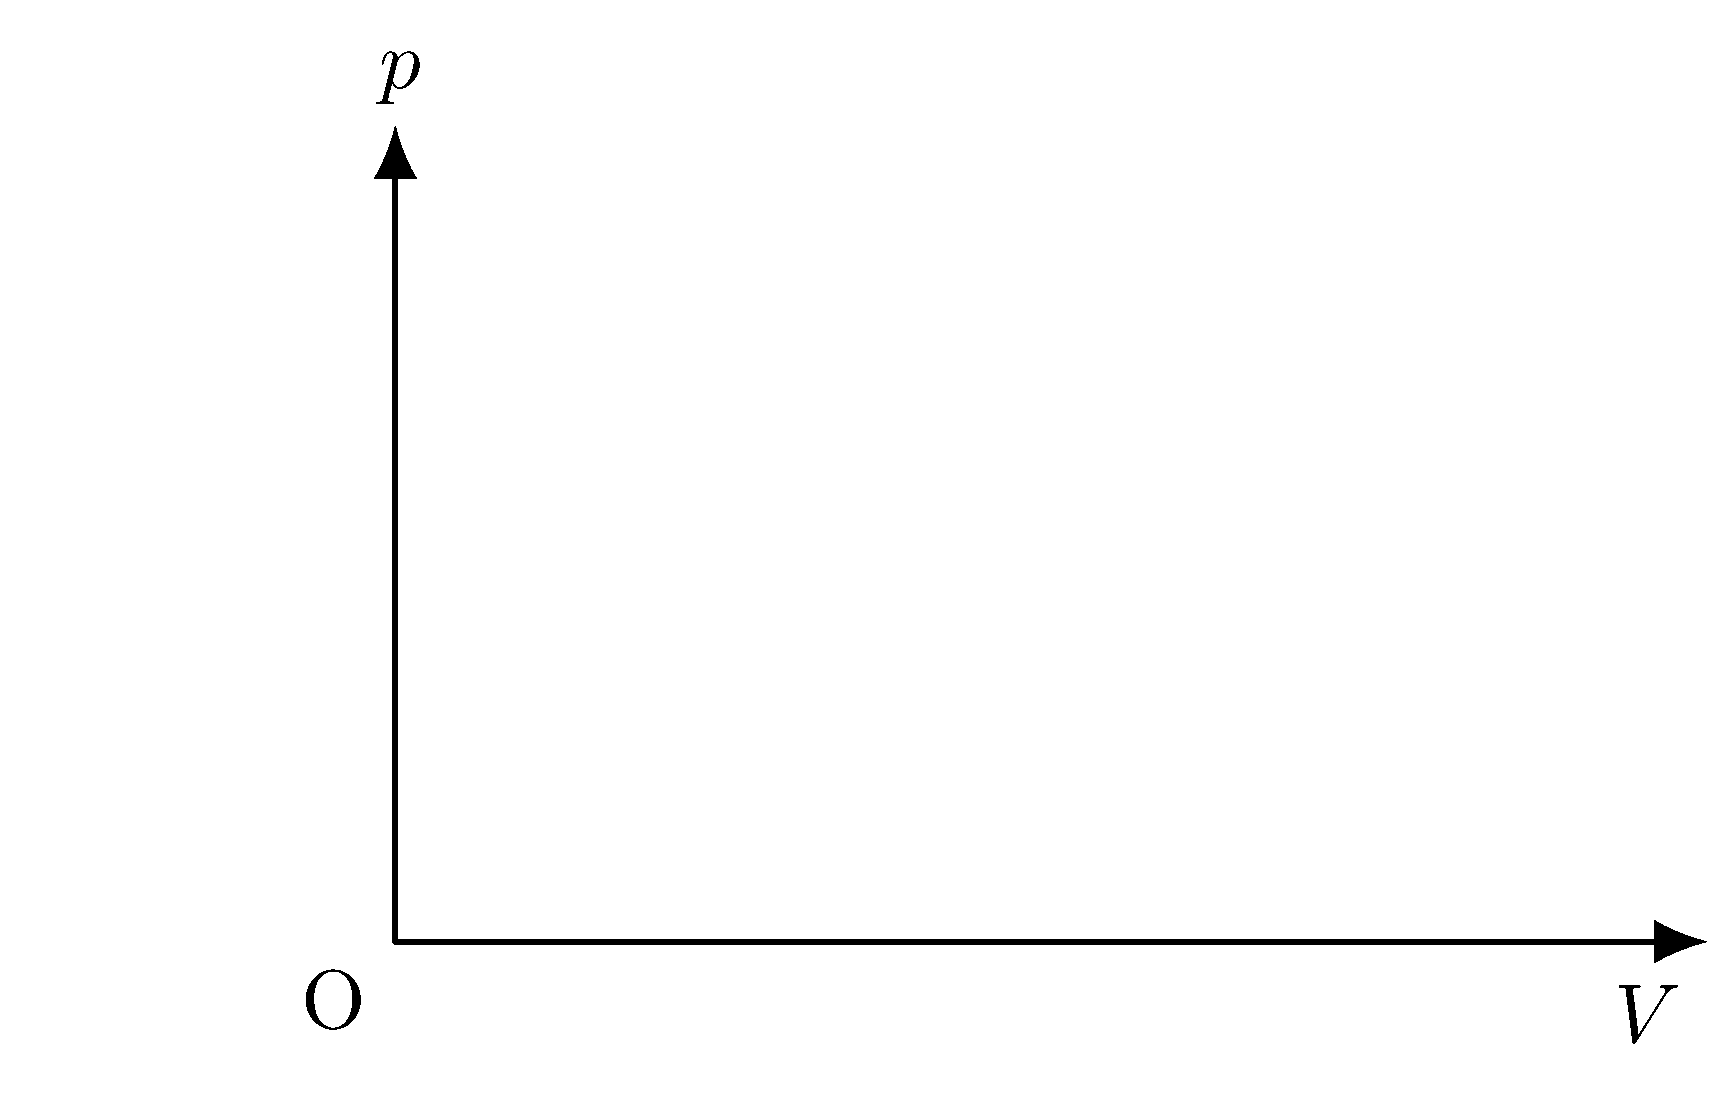
\includegraphics[keepaspectratio,width=72mm]{fig/ch16_ex8_pv_blank.png}
       \else
       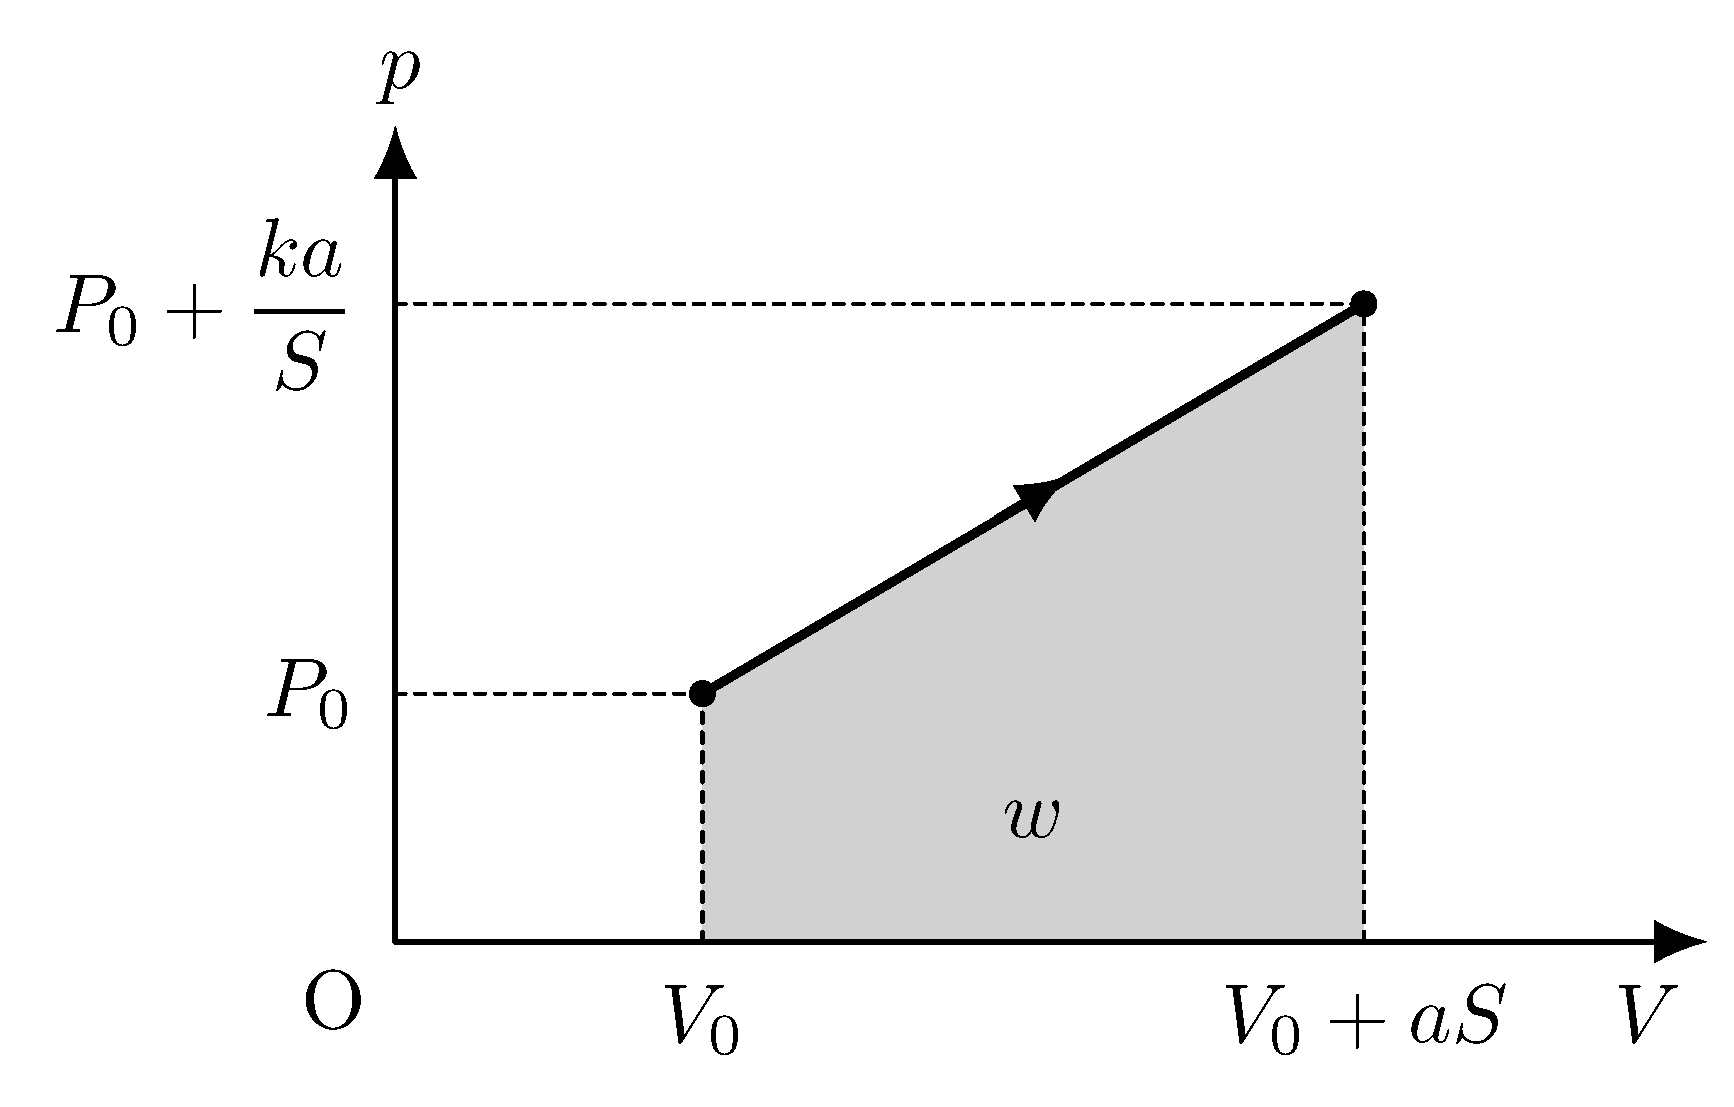
\includegraphics[keepaspectratio,width=72mm]{fig/ch16_ex8_pv.png}
       \fi
       \end{center}
       \hspace*{\fill}\Ans
\ko{4} (2)を$x:0\rightarrow a$の範囲で積分して，
       \Ana{w=\int_0^a(P_0S+kx)\,dx=P_0Sa+\frac{1}{2}ka^2\U{J}\Ans}
\end{komon}
\end{kaitou}
\end{reidaiunit}

%%%%%%%%%%%%%%%%%%%%  例題9（16.3 のまとめ枠の直後）  %%%%%%%%%%%%%%%%%%%%
\begin{reidaiunit}
\begin{reidai}{定積変化（$C_V$の物理的意味）}
\begin{zuright}{52mm}
\hspace{1zw}図のように一様な断面積を持つシリンダーに定積モル比熱が$C_V\U{J/mol\cdot K}$の理想気体を$n\U{mol}$封入し，ピストンの位置を固定して動かないようにした．\par
\hspace{1zw}最初，この気体の温度は$T_0\U{K}$，圧力は$P_0\U{Pa}$であった．
\zusep
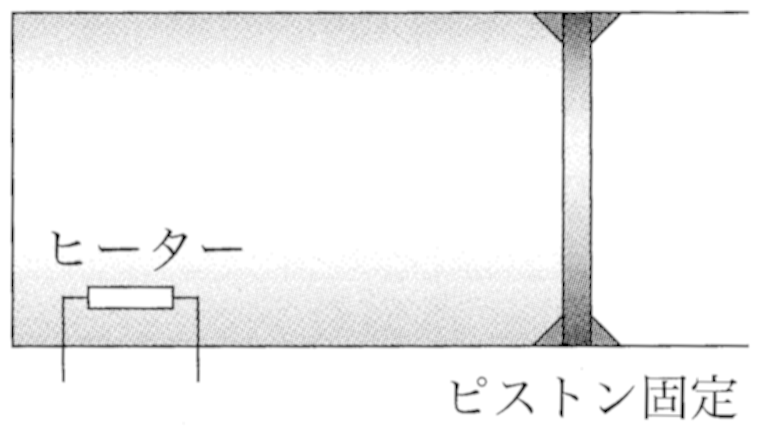
\includegraphics[keepaspectratio,width=52mm]{fig/ch16_ex9_cyl.png}
\end{zuright}
\hspace{1zw}シリンダー内にはヒーターが取り付けてあり，気体に対して熱を与えることができる．シリンダーおよびピストンは断熱材で出来ており，ヒーターによって与えた熱が大気に拡散することはないものとする．

\hspace{1zw}この状態から気体に熱をゆっくりと与え，気体の温度が$\Delta T\U{K}$だけ上昇したところで加熱を止めた．気体定数を$R\U{J/mol\cdot K}$として以下の問に答えよ．
\begin{komon}
\ko{1} この状態変化を$P-V$図で表せ．
\ko{2} この変化において気体が外界に対してした仕事$w\U{J}$を求めよ．
\ko{3} この変化における気体の内部エネルギーの増加$\Delta U\U{J}$およびヒーターによって加えた熱量$Q\U{J}$を求めよ．
\end{komon}
\end{reidai}

\begin{sisinE}
ピストンが固定されているので体積は変化しない．体積が変わらなければ気体は仕事をやり取りしないから，加えた熱はすべて内部エネルギーの増加になる．これが「定積モル比熱$C_V$の物理的意味」である．

$\Delta U=nC_V\Delta T$は定積変化に限らずあらゆる状態変化で成立する式であるが，$Q=nC_V\Delta T$の方は定積変化でしか成立しない．本問はその二つがたまたま一致する場合である．
\end{sisinE}

\Key{状態方程式 $PV=nRT$\quad $\Delta U=nC_V\Delta T$\quad $w=\displaystyle\int_{V_1}^{V_2}P\,dV$\quad $\Delta U=Q+(-w)$}

\begin{kaitou}
\begin{komon}
\ko{1} 体積が変化しないので，$P-V$図は$V$軸に垂直な線分となる．初めの状態の状態方程式$P_0V_0=nRT_0$より体積は$V_0=\dfrac{nRT_0}{P_0}\U{m^3}$，終状態の状態方程式$P_1V_0=nR(T_0+\Delta T)$より圧力は$P_1=\dfrac{T_0+\Delta T}{T_0}P_0\U{Pa}$であり，加熱したので圧力は上昇する．よって$P-V$図は次図．
       \begin{center}
       \ifbsAnaume
       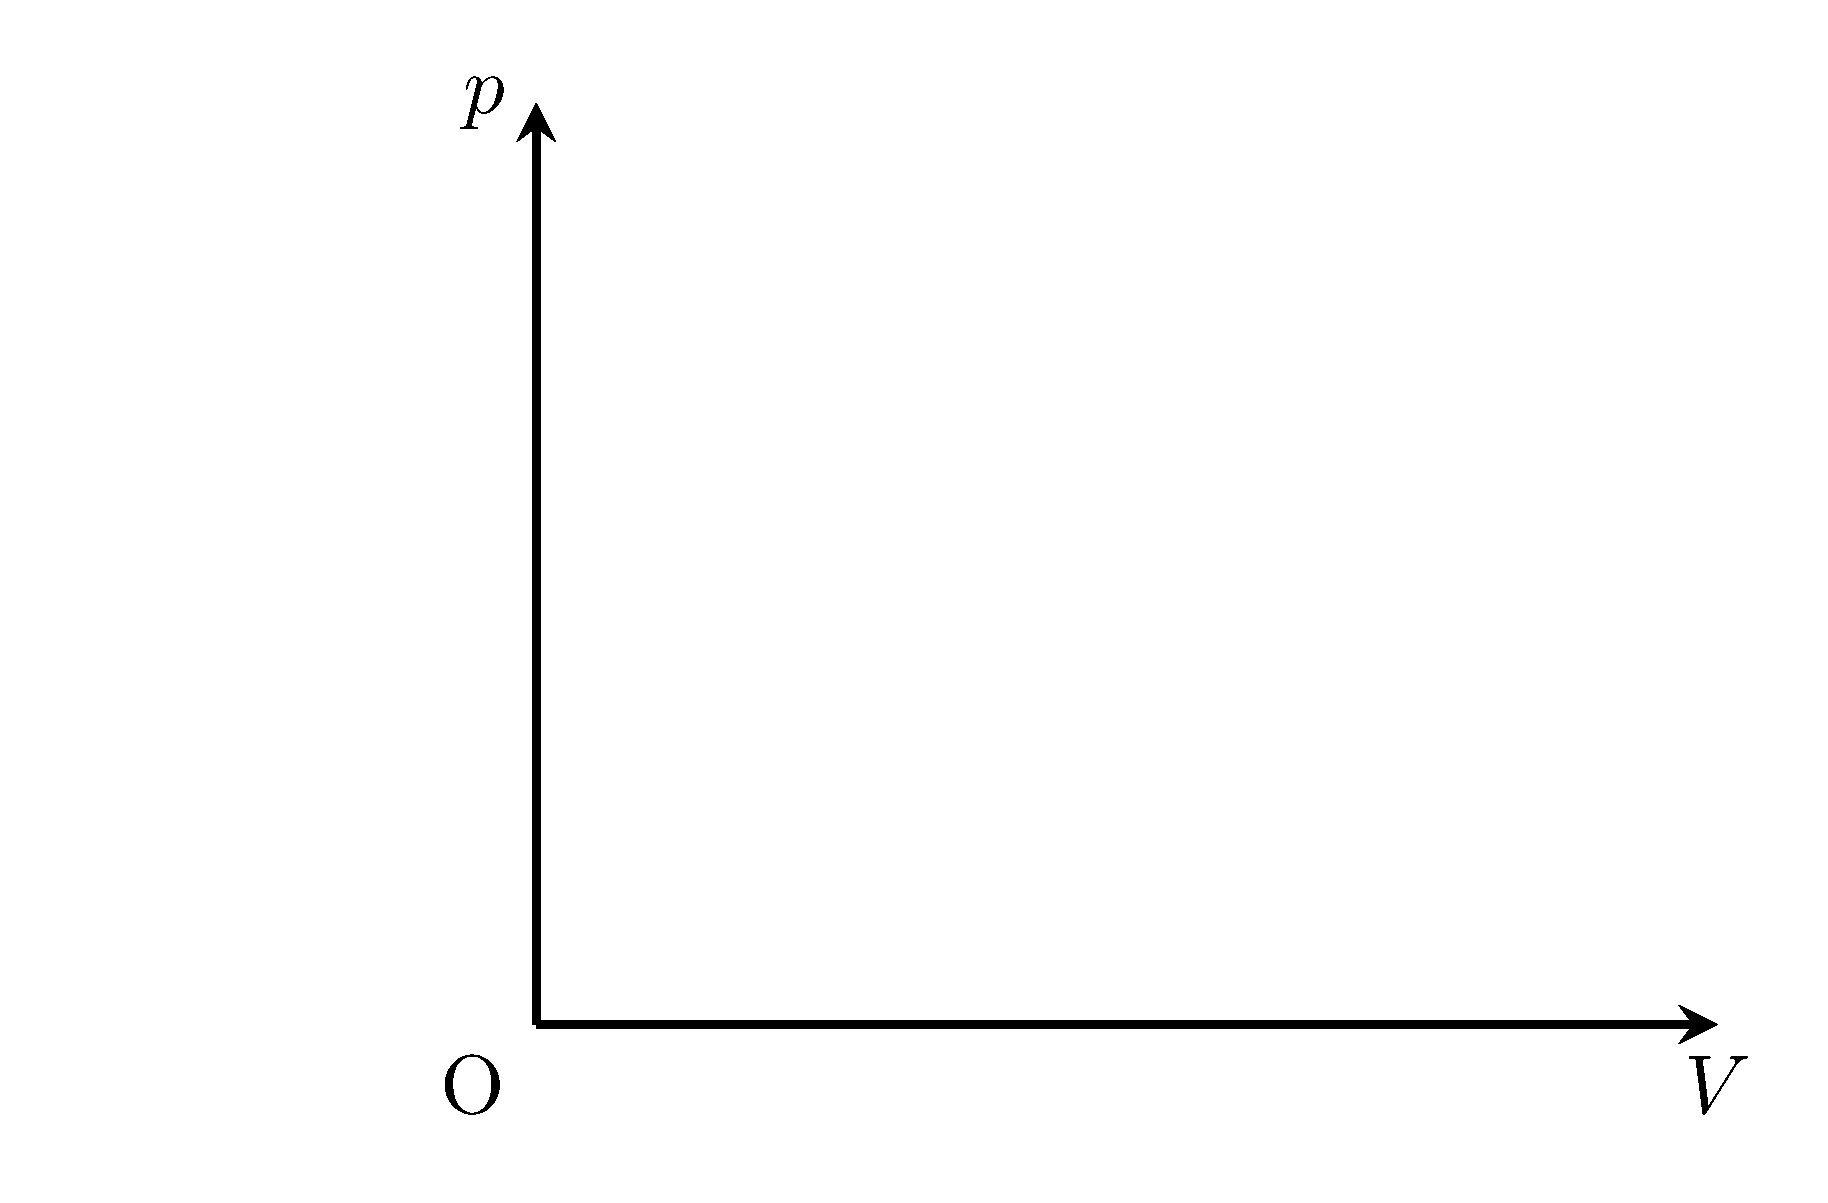
\includegraphics[keepaspectratio,width=72mm]{fig/ch16_ex9_pv_blank.png}
       \else
       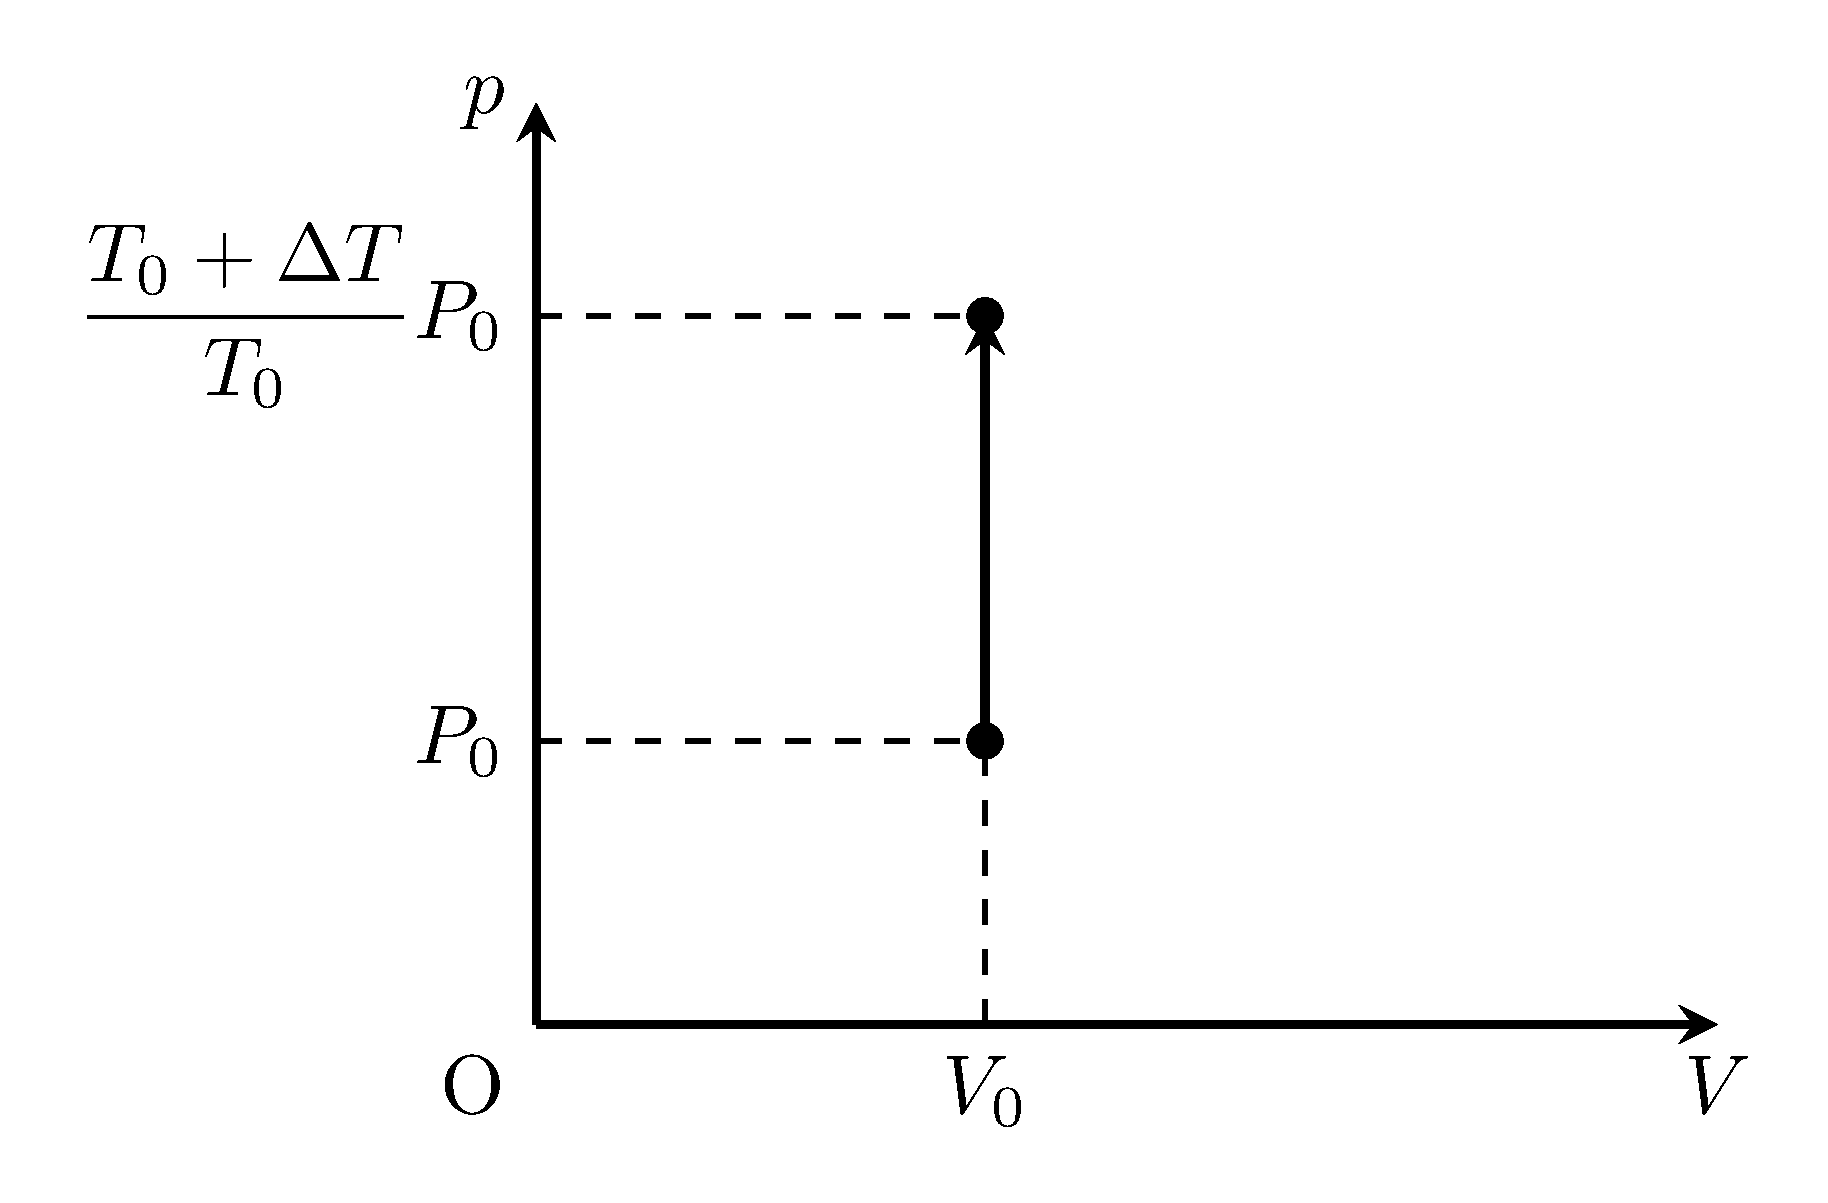
\includegraphics[keepaspectratio,width=72mm]{fig/ch16_ex9_pv.png}
       \fi
       \end{center}
       \hspace*{\fill}\Ans
\ko{2} 体積変化がないので，気体は外界に対して仕事をしない．
       \Ana{w=\int_{V_0}^{V_0}P\,dV=0\U{J}\Ans}
\ko{3} 内部エネルギーの変化は状態変化の種類によらず$\Delta U=nC_V\Delta T$と書けるので，
       \Ana{\Delta U=nC_V\Delta T\U{J}\Ans}
       また，熱力学第一法則$\Delta U=Q+(-w)$と(2)より，
       \Ana{Q=\Delta U+w=nC_V\Delta T\U{J}\Ans}
\end{komon}
\end{kaitou}
\end{reidaiunit}

%%%%%%%%%%%%%%%%%%%%  例題10（例題9 の直後）  %%%%%%%%%%%%%%%%%%%%
\begin{reidaiunit}
\begin{reidai}{定圧変化}
\begin{zuright}{52mm}
\hspace{1zw}図のように一様な断面積を持つシリンダーに定積モル比熱が$C_V\U{J/mol\cdot K}$の理想気体を$n\U{mol}$封入した．ピストンは軽くて自由に動くことができ，大気圧$P_0\U{Pa}$とシリンダー内の気体の圧力とが常につり合いを保つ．最初，この気体の温度は$T_0\U{K}$であった．
\zusep
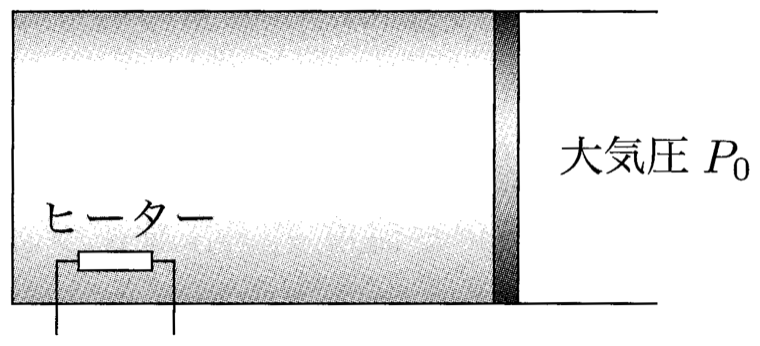
\includegraphics[keepaspectratio,width=52mm]{fig/ch16_ex10_cyl.png}
\end{zuright}
\hspace{1zw}シリンダー内にはヒーターが取り付けてあり，気体に対して熱を与えることができる．シリンダーおよびピストンは断熱材で出来ており，ヒーターによって与えた熱が大気に拡散することはないものとする．気体定数を$R\U{J/mol\cdot K}$として以下の問に答えよ．
\begin{komon}
\ko{1} 初めの状態における気体の体積$V_0\U{m^3}$を求めよ．
\end{komon}
\hspace{1zw}この状態から気体に熱をゆっくりと与え，気体の温度が$\Delta T\U{K}$だけ上昇したところで加熱を止めた．
\begin{komon}
\ko{2} この変化における気体の内部エネルギーの増加$\Delta U\U{J}$を求めよ．
\ko{3} この変化における気体の体積増加$\Delta V\U{m^3}$を求めよ．
\ko{4} この状態変化を$P-V$図で表せ．
\ko{5} この変化において気体が外界に対してした仕事$w\U{J}$を求めよ．
\ko{6} ヒーターによって加えた熱量$Q\U{J}$を求めよ．
\ko{7} (6)より，定積モル比熱$C_V\U{J/mol\cdot K}$と定圧モル比熱$C_P\U{J/mol\cdot K}$との間にマイヤーの関係式$C_P-C_V=R$が成立していることを示せ．
\end{komon}
\end{reidai}

\begin{sisinE}
ピストンが軽くて自由に動くので，気体の圧力は常に大気圧$P_0$に等しい．すなわち定圧変化である．

(5) 定圧変化の場合，$w=\displaystyle\int_{V_1}^{V_2}P\,dV$の式の$P$は$V$によらず一定であるから，積分の外に出して扱うことが出来る．すなわち，$w=P\Delta V$とできる．
\end{sisinE}

\Key{状態方程式 $PV=nRT$\quad $\Delta U=nC_V\Delta T$\quad $w=\displaystyle\int_{V_1}^{V_2}P\,dV$\quad $\Delta U=Q+(-w)$}

\begin{kaitou}
\begin{komon}
\ko{1} 初めの状態の状態方程式$P_0V_0=nRT_0$より，
       \Ana{V_0=\frac{nRT_0}{P_0}\U{m^3}\Ans}
\ko{2} 内部エネルギーの変化は状態変化の種類によらず，
       \Ana{\Delta U=nC_V\Delta T\U{J}\Ans}
\ko{3} 終状態の状態方程式は$P_0(V_0+\Delta V)=nR(T_0+\Delta T)$である．これと(1)の状態方程式の差をとって，
       \Ana{P_0\Delta V=nR\Delta T}
       よって，
       \Ana{\Delta V=\frac{nR\Delta T}{P_0}\U{m^3}\Ans}
\ko{4} 圧力が$P_0$のまま一定で，体積が$V_0$から$V_0+\Delta V$へ増加するので，$P-V$図は次図．
       \begin{center}
       \ifbsAnaume
       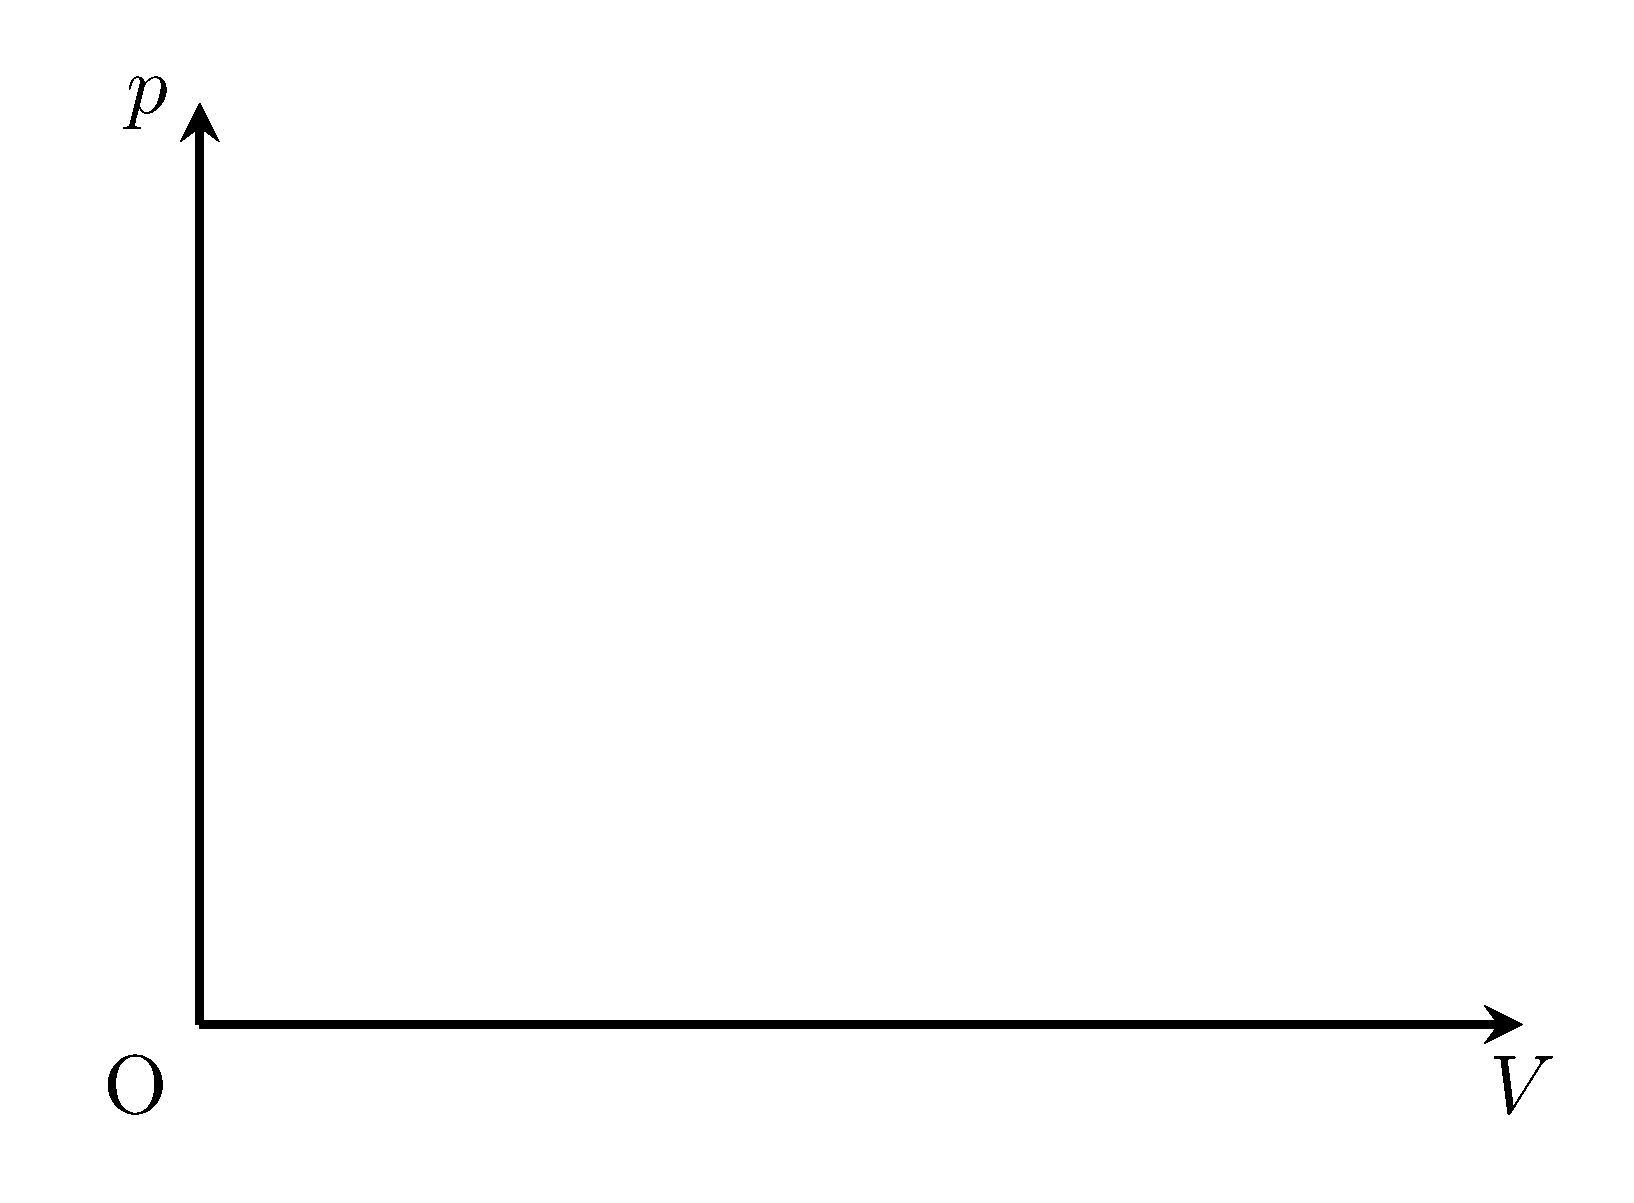
\includegraphics[keepaspectratio,width=72mm]{fig/ch16_ex10_pv_blank.png}
       \else
       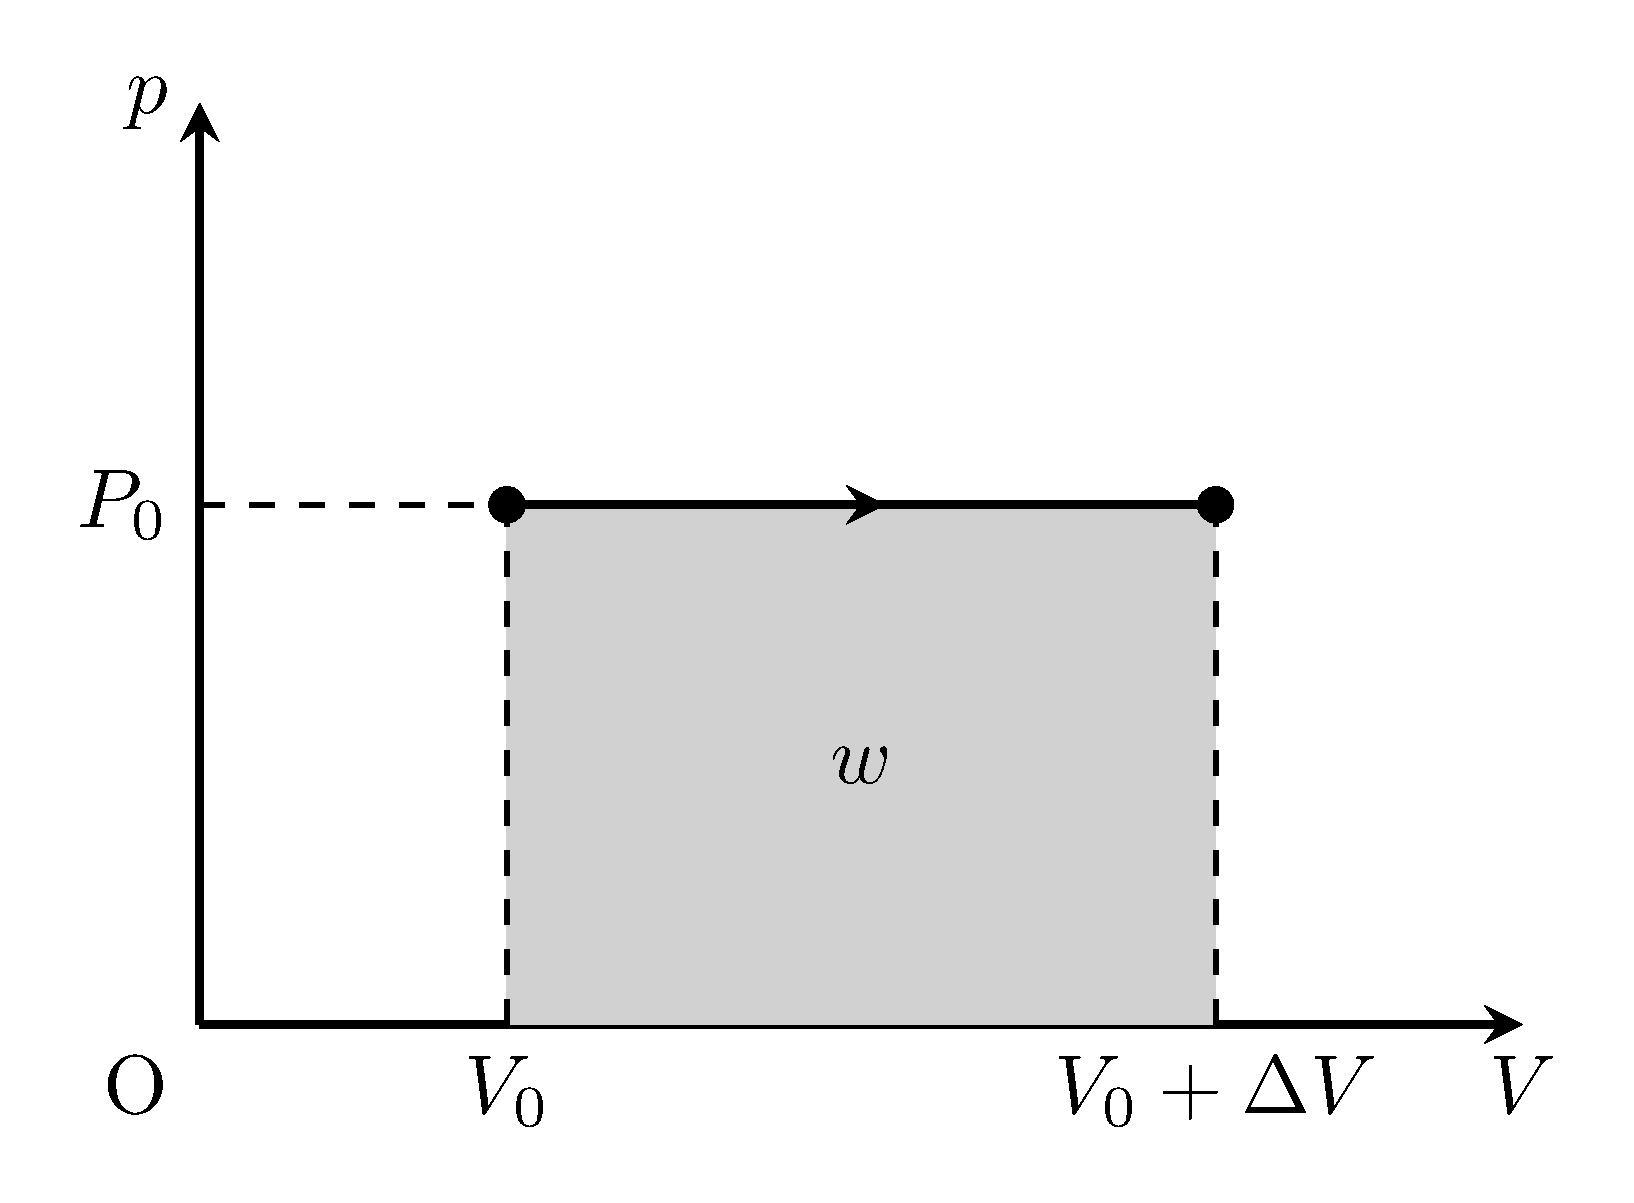
\includegraphics[keepaspectratio,width=72mm]{fig/ch16_ex10_pv.png}
       \fi
       \end{center}
       \hspace*{\fill}\Ans
\ko{5} 定圧変化であるから$P_0$を積分の外に出して，
       \Ana{w=\int_{V_0}^{V_0+\Delta V}P_0\,dV=P_0\Delta V=nR\Delta T\U{J}\Ans}
\ko{6} 熱力学第一法則$\Delta U=Q+(-w)$より，(2)(5)を代入して，
       \Ana{Q=\Delta U+w=n(C_V+R)\Delta T\U{J}\Ans}
\ko{7} この状態変化は定圧変化であるから，定圧モル比熱の定義より$Q=nC_P\Delta T$とも書ける．これと(6)を比べて，
       \Ana{nC_P\Delta T=n(C_V+R)\Delta T}
       $\Delta T\neq 0$であるから両辺を$n\Delta T$で割って$C_P=C_V+R$，すなわち
       \Ana{C_P-C_V=R}
       が成立する．
\end{komon}
\end{kaitou}
\end{reidaiunit}
